\documentclass{article}

\usepackage{a4}
\usepackage{setspace}
\usepackage{graphicx}

\title{A Deeper Understanding of the s-Process:\\
A Ph.D. Oral Qualifier}
\author{by: Jaad A. Tannous\\
Advisor: Prof. Bradley S. Meyer}
\date{}

\begin{document}
\maketitle

\section*{Abstract}
The aim of this document is to provide the committee a quick recap of the s-process, and how I aim to 
contribute to further its understanding. The first section is a brief recap, but granted not a complete 
one, on the s-process. The following four will outline tools being developed, and aspects that are being 
studied. In the last section I will conclude how the project will come together.

\section*{The s-process}
The slow neutron capture process, s-process, is a series of reactions in nuclear astrophysics that is responsible 
for synthesizing half the elements heavier than iron. It occurs in moderately neutron rich environments and requires 
existing iron as a seed nucleus. The reactions involved are a series of neutron captures and $\beta^{-}$ decays. Heavier 
isotopes will form until one that is $\beta$ unstable is reached, and its decay rate is shorter than the capture rate; as illustrated 
in Fig. 1.

\begin{figure}[!htp]
    \centerline{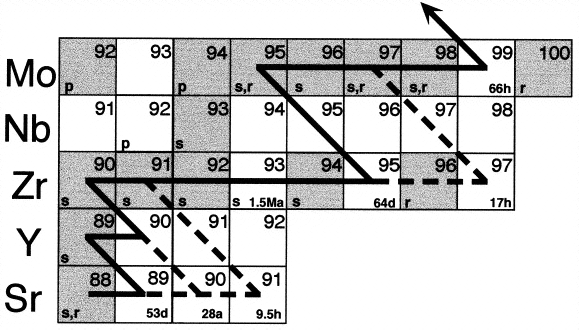
\includegraphics[scale = 0.5]{images/sprocess.png}}
    \caption{A Z-N flow chart illustrating a cut of s-process nucleosynthesis from Strontium up till 
    Molybdenum. The solid line indicates the main path, while the dotted a secondary branch.\cite{nic98}}
\end{figure}

\noindent It is a slow process because the $\beta^{-}$ decays occur on shorter timescales than the next neutron capture. In comparison, 
neutron captures may take days or years, while beta decays can take between seconds and hours.

\subsection*{Main s-process}


\section*{Neutron Exposure}
\section*{Isomers}
\section*{T and $Y_{e}$ dependent rates}
\section*{Multizone framework development}
\section*{My research}

\singlespacing

\bibliographystyle{apalike}
\bibliography{references.bib}

\end{document}